\documentclass[11pt]{article}
\usepackage{amsmath}
\usepackage{graphicx}
\usepackage{float}
\usepackage{blindtext}
\usepackage{subcaption}
\usepackage[a4paper,margin=2cm]{geometry}
\usepackage{fancyhdr}
\usepackage{longtable}
\usepackage[
    backend=biber,
    style=ieee
]{biblatex}
\usepackage{xcolor}
\usepackage{soul}
\usepackage{listings}

\newcommand{\hlc}[2][yellow]{{%
    \colorlet{foo}{#1}%
    \sethlcolor{foo}\hl{#2}}%
}


\addbibresource{report.bib}

\graphicspath{ {./images/} }

\pagestyle{fancy}
\fancyhead[C]{Report}
\fancyhead[L]{EEE3027 Calculator Assignment}
\fancyhead[R]{2nd of May}

\cfoot{} % get rid of the page number 
\fancyfoot[L]{6596386}
\fancyhead[C]{}
\fancyfoot[R]{\thepage}

\begin{document}
\begin{titlepage}
    \begin{center}
    
\includegraphics[width=\textwidth]{Logo.png} % also works with logo.pdf
    \vfill
    \Huge
    \textbf{EEE3027: Calculator Assignment}
    \vfill
    \huge
    Assignment Report\\
    \vspace{1cm}
    \Large
    2nd of May 2023\\
    URN: 6596386\\
    \vfill
    \vfill
    \Large
    Department of Electronic Engineering\\
    Faculty of Engineering and Physical Sciences\\
    University of Surrey\\
    \end{center}
\end{titlepage}

\begin{abstract}
This report covers the work done on creating and testing an FPGA Calculator in VHDL as part of EEE3027 Digital Design with VHDL.
VHDL was used to program an FPGA capable of taking serial input,
converting the serial input to numbers and operations,
calculating the result,
converting the result back into serial, 
and finally transmitting the result back.
The final design allows for a user to input, over serial, any integer between -32767 and 32767 (a signed 16-bit value) with the following integer operation : addition, subtraction, multiplication, and division. 
The FPGA will then return the result if it can be represented as a signed 16-bit value, otherwise it will return an error. 
The report also covers background theory for UART communication, an exploration of the original provided code, and a discussion on timing and physical implementation on a Minized Zynq board.
\vspace{1cm}
\end{abstract}
\tableofcontents
\pagebreak

\section{Overview}

The objectives of this assignment were to create an arithmetic calculator using the std.numeric library and provided UART code.
This provided code first has to be debugged and tested.
The calculators basic requirement was to compute values given in the "$A {+-*/} B$" format, with no specific instructions of the range of values of $A$, $B$ or the output.
For the implementation created for this assignment the calculator is able to take inputs and provide outputs that can be described as signed 16-bit integers (ie between -32767 and 32767),
however, through the use of generics this range can be changed.
The serial UART input is then processed into the two expected numbers and operations, with any character that is not a numeral (0 to 9) or an operator character ($+-*/$) being ignored.
At the end of the input a carriage return character (ASCII Hex code $0D$) is required to indicate the end of number $B$.
A carriage return is also transmitted at the end of the calculator response with the result.
Furthermore the final design will output a special character, "!", when an operation is invalid (such as dividing by zero) or the output is outside the calculators range.

\begin{figure}[H]        
    \centering
    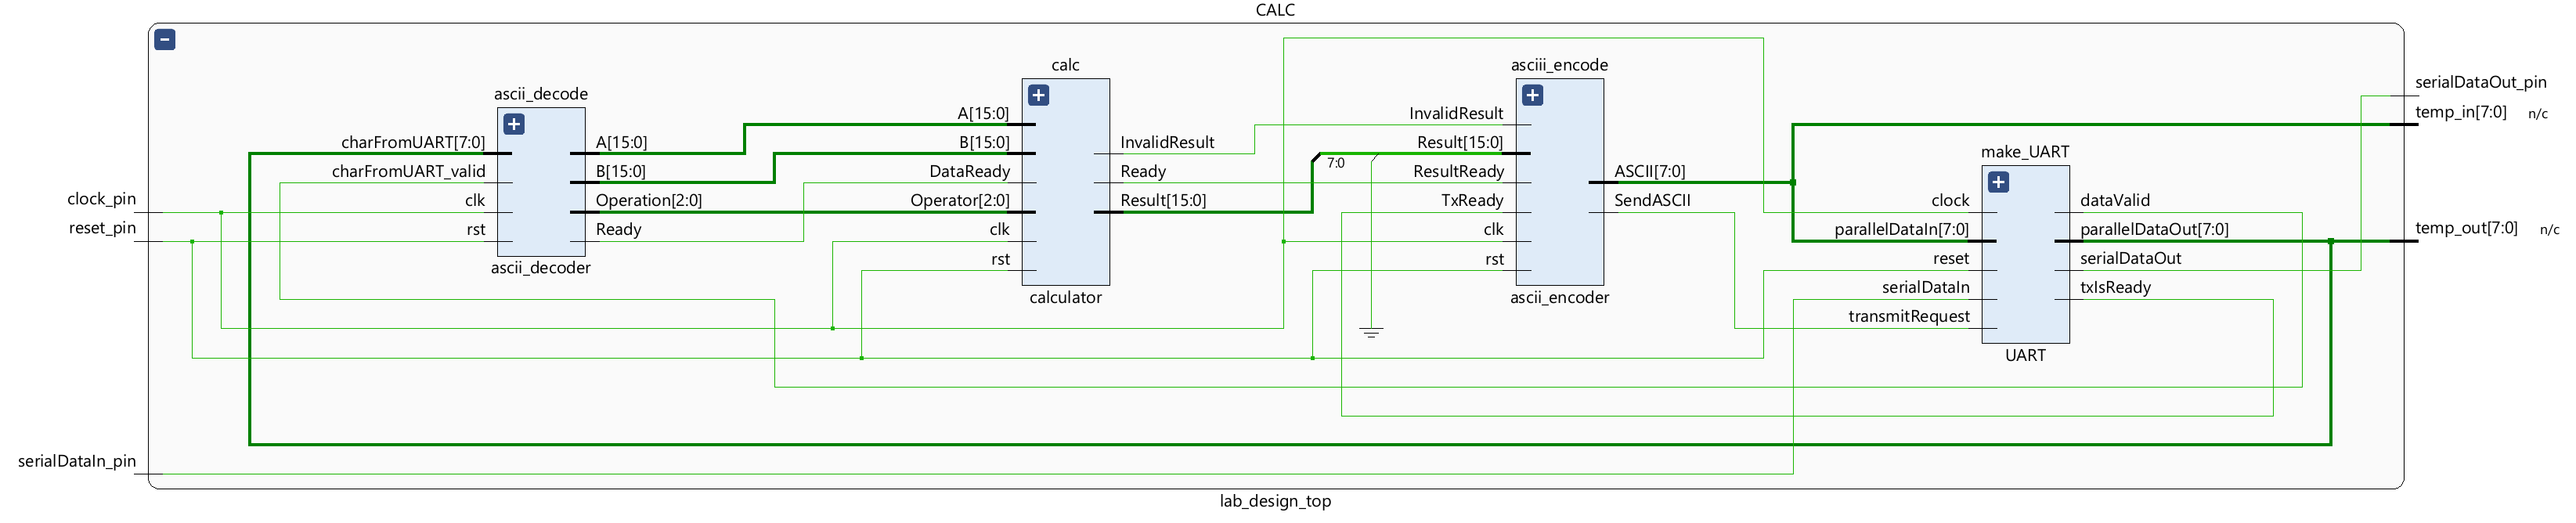
\includegraphics[width=\textwidth]{TopLevelImp.png}
    \caption{Top Level Implementation of Calculator}
    \label{fig:toplevel}
\end{figure} 

To achieve this functionality the design seen in figure \ref{fig:toplevel} was created, with four main components all interacting together.
These components are the UART block, the ASCII decoder, the calculator, ASCII encoder.
The UART block handles the receiving of serial UART data and converting it to parallel data as well as taking parallel data and sending it as serial UART.
The ASCII decoder takes the parallel data, assuming they are ASCII codes, and converts into two numbers and a operation.
The calculator computes operations between two numbers, the provides a result as well as a signal if the operation is invalid.
THe ASCII encoder takes a result, as well the invalid signal, and converts them into a sequences of parallel ASCII codes that it sends to the UART block.
Details on the design and operation of all of these components, as well information on testbenches and implementation on a Minized Zynq FPGA board are provided in


\section{UART}
\subsection{UART Theory}
UART stands for universal asynchronous receiver-transmitter and is a very common device-to-to device communication protocol\cite{UART}.
For this assignment a two-way UART connection is utilized,
allowing two devices (the FPGA and a connected PC) to transfer data between each other regardless of clock rate as long as they communicate over a predefined rate know as the baud rate.
Unlike other communication protocols such as SPI or I2C, UART only ever has one "master" device and one "slave" device a third device cannot be added on the same lines.

UART takes parallel data and converts it into a bit by bit frame to send.
The frame always start with the start bit, which takes the line low for one cycle as UART is normally high.
then each data bit is sent one by one (least significant bit first) with a 1 being high and a zero being low.
Some implementation will include a parity bit after the data, which will be 0 if the data total is odd and 1 is the total is even.
Parity is useful to ensure that data been altered during transmission, which can occur due to "electromagnetic radiation, mismatched baud rates, or long-distance data transfers"\cite{UART}.
The provided UART however does not utilize the parity bit.
At the end of the message a stop bit is sent going from low to high.
Equation \ref{eq:uart_sample} shows an example of how data gets converted to 

\begin{align*}
    \text{Data} &= 01000001
    \stepcounter{equation}\tag{\theequation}\label{eq:uart_sample} \\
    \text{UART Frame} &=    \overset{\text{Start Bit}}{\{0\}}
                            \underset{\text{Data}}{\{1000 0010\}}
                            \overset{\text{Stop Bit}}{\{1\}}\\
\end{align*}


The final key concept behind UART is the baud rate, which the number of signals per second.
In the case of UART baud rate represents how long each bit is held high or low.
As UART is asynchronous, each device needs to know baud rate ahead of time and generate its own clock at the baud rate.
This is enough to transmit UART as the line can simply be updated each clock cycle,
however for receiving the line needs to be checked more often as the devices baud clocks can be out of phase by half a period and because reals signal have non-instantaneous transition periods from high to low meaning that is best to check the signal in the middle of each cycle.
To do this there is a secondary oversampled clock, oven 16x, that is used in the receiver to check in the middle of each received by instead.
Then when a start bit is received the receiver will wait for roughly half a baud to sample the next bit.
After this point the the receiver will wait 16 of the oversampled rates to take the next sample.
Some implementations may take multiple samples around the midpoint to get a more accurate result, however this implementation takes only one measurement.
Once enough measurements have been made, something else that needs to be predefined, the receiver will wait for the stop bit.

% This method of having both receiver and transmitter create their own baud clock means that communication occurs without a shared clocked, letting devices running at vastly different frequencies communicate.
% Ideally when each device will perfectly generate a clock for baud allowing for flawless communication even when the receiver and transmitter are completly out of phase (ie half a baud period apart), however the baud rates a device can support are limited by its own clock.
% As the smallest unit of time a device can use is a clock period the actual baud rate may differ from the desired baud rate.
% For example with a 60 MHz clock the smallest unit is 16.66 ns, and to create a 115.2 kHz baudrate a 8680.56 ns period is required which can be approximated with 521 clock cycles (which is 8683.33 ns).
% This  means the acutal baudrate will be  115.207373 \cite{baudrate}

\subsection{UART Component}
\begin{figure}[H]        
    \centering
    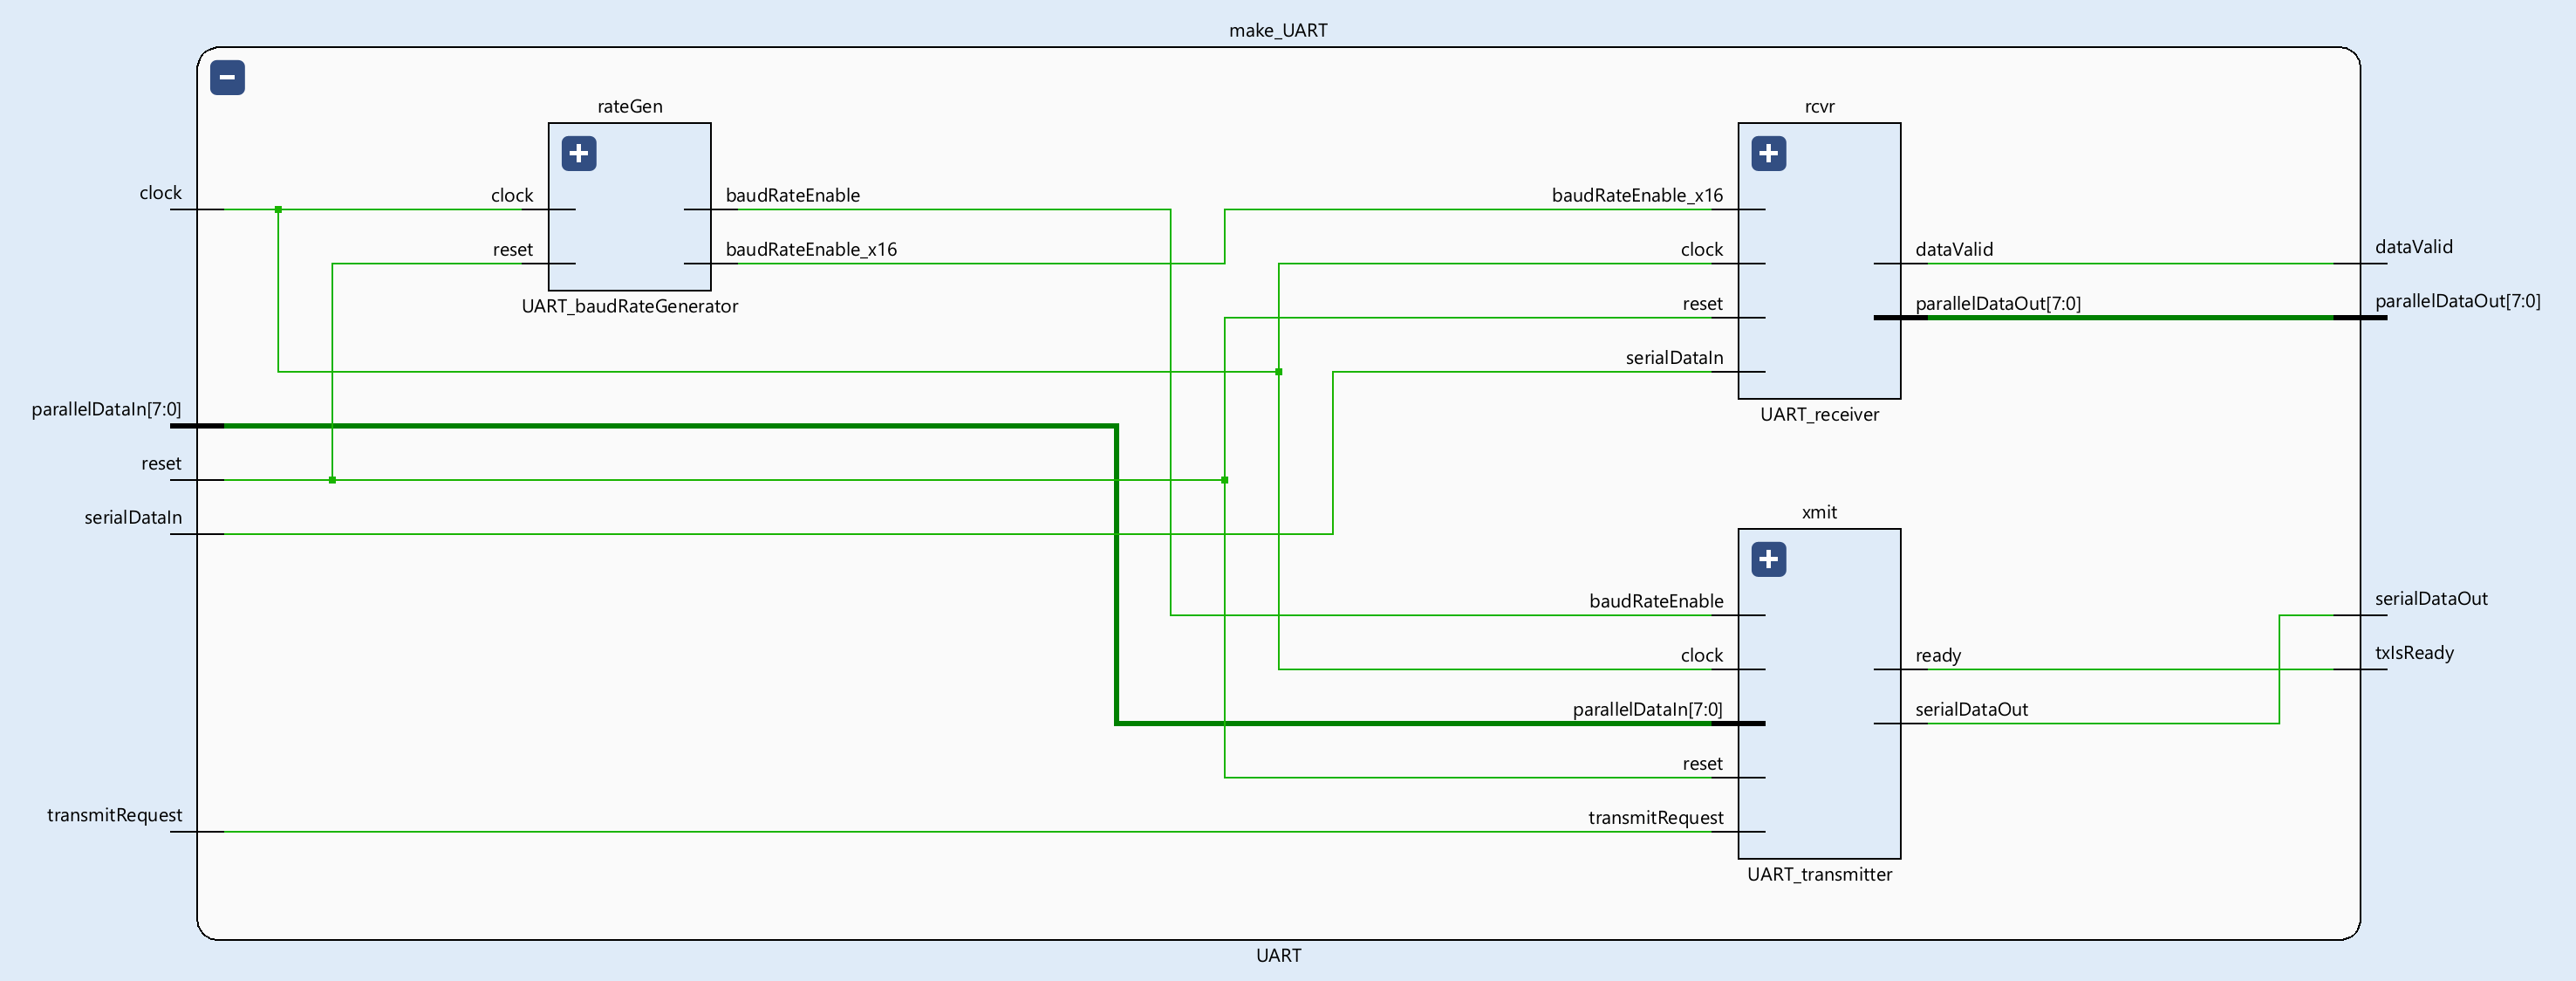
\includegraphics[width=\textwidth]{uartImp.png}
    \caption{UART Block Diagram}
    \label{fig:UARTimp}
\end{figure} 

Provided with the assignment was the VHDL code for a UART transmitter and receiver. 
This code required a few corrections to get in working order. 
The simpler of the fixes was that all files required the addition of the IEEE std\_logic\_1164 library. 
Testing also revealed that the UART receiver was not connected to the baudRateEnable\_x16 line which was quickly fixed in the port map.
The baud rate generator also had the incrementing of its baud counts moved with-in the if statements to avoid incrementing the variable and then instantly setting it to zero, in order to keep this from breaking the timing the check for completion was also altered.
With the fixes the components functioned as expected.

This means that the baud rate generator given a clock line and predefined with the clock frequency and desired baud rate will produce two outputs: a pulse at the baud rate and a pulse at 16 times the baud rate which connect to the transmitter and receiver respectively.
It does this by counting an the number of clock cycles and sending a pulse every x cycles and resetting the count, where x is the clock rate over the baud rate.
The baud rate transmitter takes five inputs, a clock, a reset, baud pulses, a transmit request and an 8-bit bus for the output date.
Every clock cycle it will check if the transmit request is high, once it is it will begin to send a UART message including start and stop bit containing the data that was on 8-bit bus when the transmits request was received.
This operation is achieved using a finite state machine, a diagram for which can be seen in figure \ref{fig:transmitsm}

\begin{figure}[H]        
    \centering
    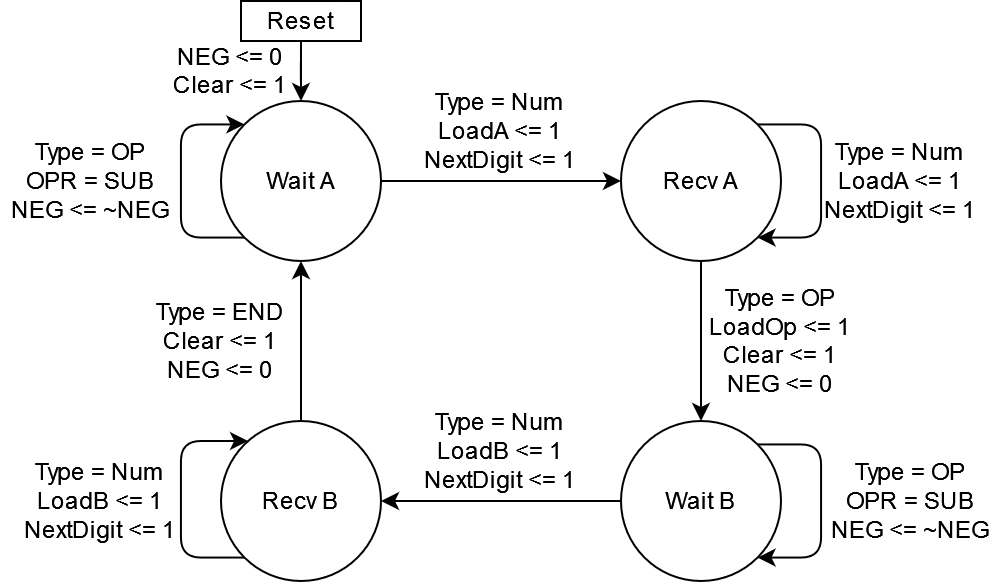
\includegraphics[width=.66\textwidth]{DecoderSM.drawio.png}
    \caption{UART Transmitter State Machine Diagram}
    \label{fig:transmitsm}
\end{figure} 

This diagram shows all the states, transitions and condition for transitions, as well as the outputs in those states and transitions. 
As the output depends both on the states and inputs, this is known as a Mealy state machine.
The $=$ sign indicates a conditions, with $<=$ being used when signals are set and $:=$ when variables are being set, this format will be used throughout the report.
Note that for this component the transition will occur only on the rising edge of baud pulses, not during the rising edge of clocks. 
The exception to this is the transmit request, which is monitored on clock rising edge and is essentially stored in a buffer as "go".
With the state machine the component will send out valid UART messages

The UART receiver takes in only a clock, a reset, and the oversampled baud pulses.
As an output it will give an 8-bit bus of data and a signal when the data is ready.
This operation is once more achieved with a state machine, seen in figure \ref{fig:receivesm}

\begin{figure}[H]        
    \centering
    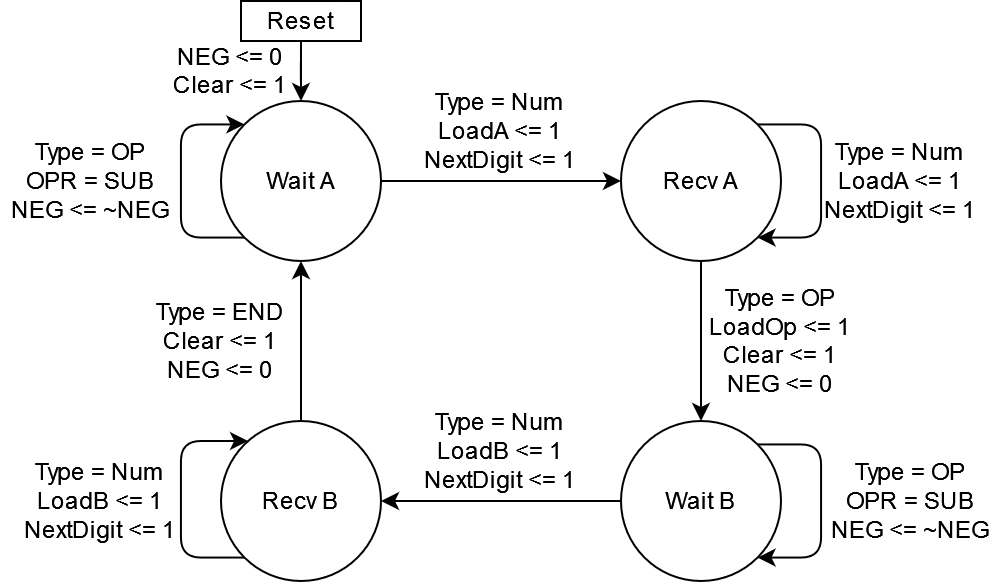
\includegraphics[width=.66\textwidth]{DecoderSM.drawio.png}
    \caption{UART Receiver State Machine Diagram}
    \label{fig:receivesm}
\end{figure} 

The core operation is similar, however as mentioned during the theory discussed the receiver makes use of a 16 times oversampled baud rate in order to take samples in the middle of data.
To achieve this the state machine transitions are triggered somewhat differently,
whenever the internal "countLoad" signal goes high the receiver will start counting up on a signal called "countValue" every oversampled baud rate and then often this count value will be used to govern what action the state machine takes next.

\subsection{Test Bench}
In order to test the UART module a simple test bench was created

\section{Original Design}
The original design, after correcting a few errors, did the following:

\section{UART Calculator}
This original design was heavily modified, with the original encoder being fully removed and the decoder being drastically changed, in order to meet the requirements for this assignment.
Figure \ref{fig:toplevel} shows this modified design.
As the UART components remains unchanged it will not be discussed again.
The overall design has three inputs: the clock, a reset line and the UART in, and only one output: the UART out.
Additionally there are four key generics: the clock rate, the baud rate, the maximum integer value, and the minimum integer value.
The first two values are used only by the UART component so that the baud pulses can be generated properly,
the integer range on the other will somewhat dynamically create version of the calculator cable of handling larger integers.
In practice the limit is -32767 to 32767, larger values may work in simulation but timing constraints prevent them from being implemented on physical hardware.


\subsection{ASCII Decoder}
% \begin{figure}[H]        
%     \centering
%     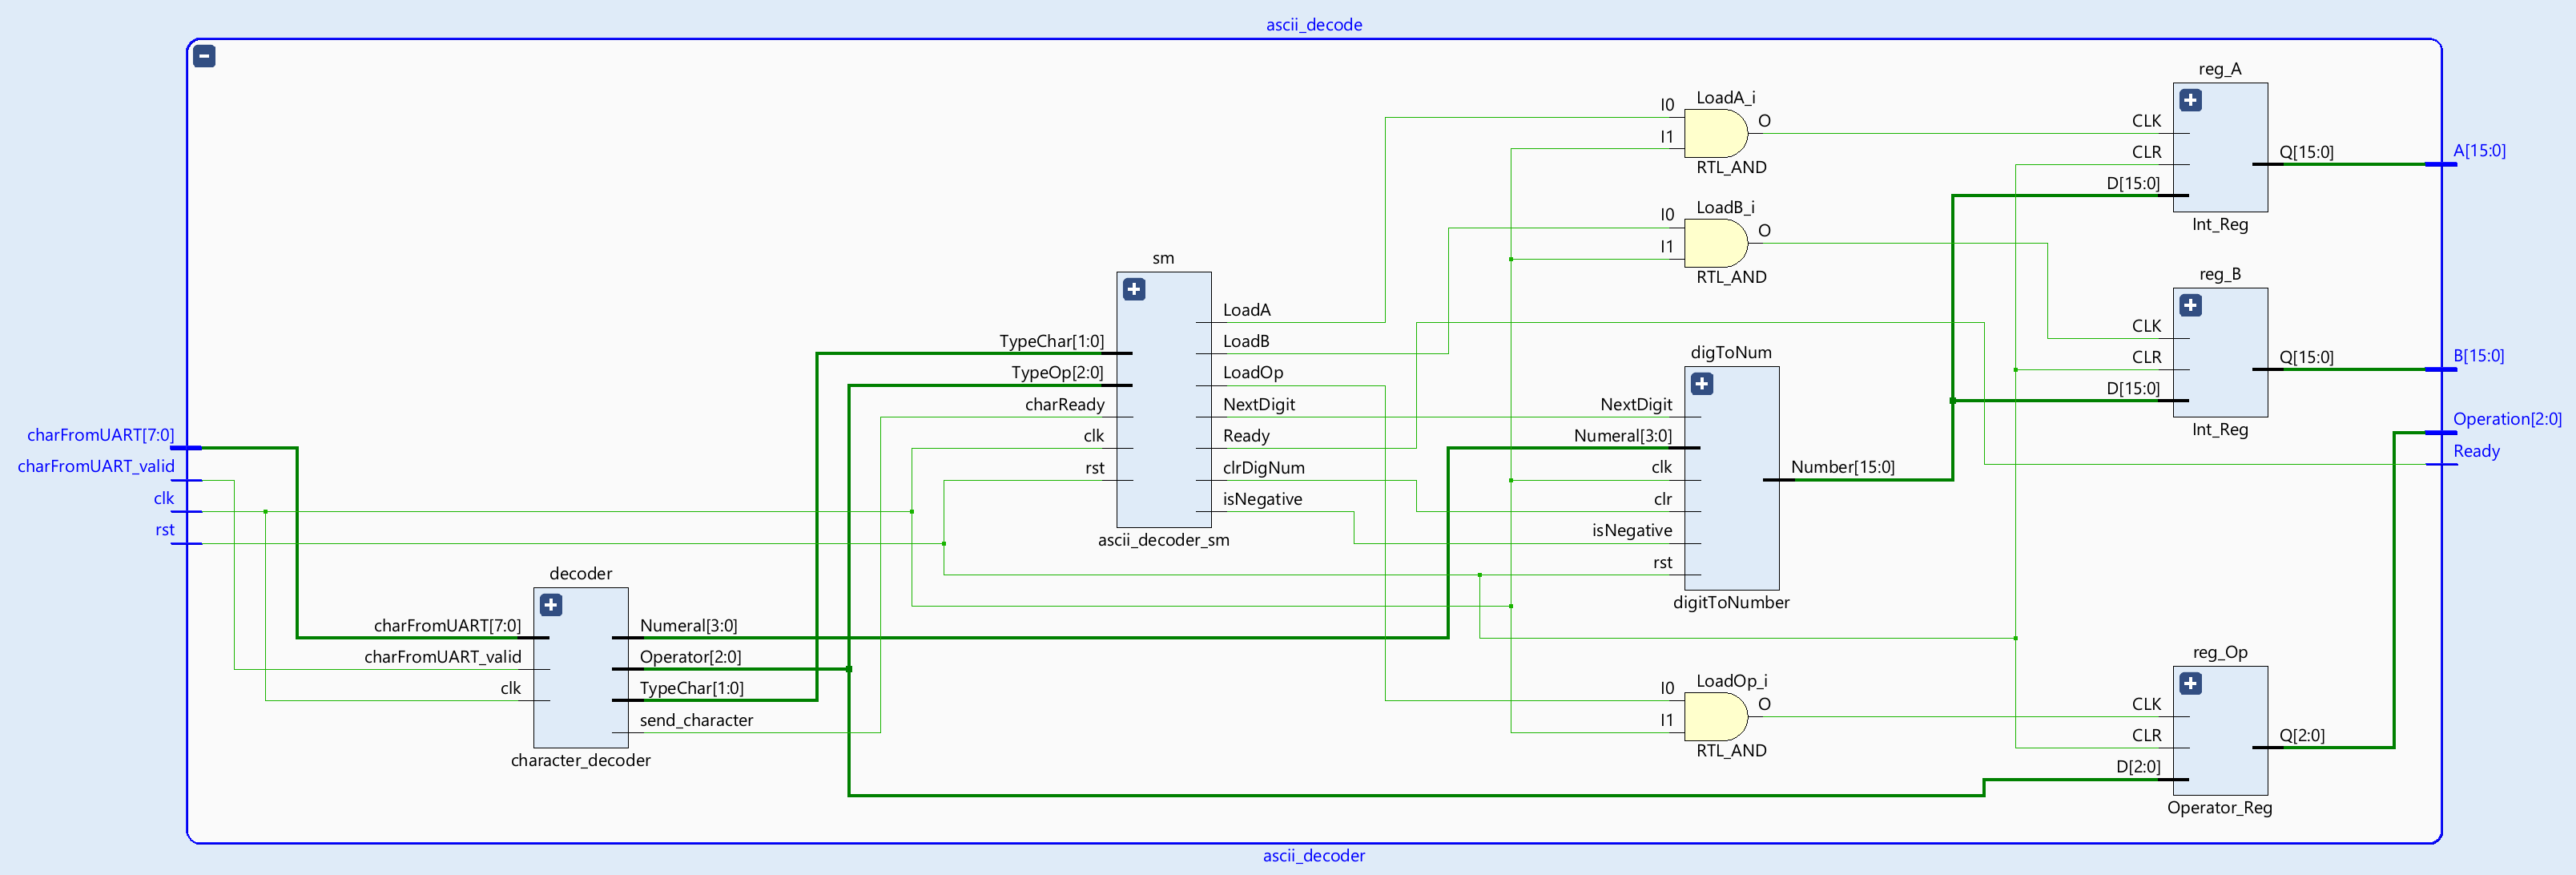
\includegraphics[width=\textwidth]{DecodeImp.png}
%     \caption{ASCII Decoder Block Diagram}
%     \label{fig:decoderimp}
% \end{figure} 

\begin{figure}[H]        
    \centering
    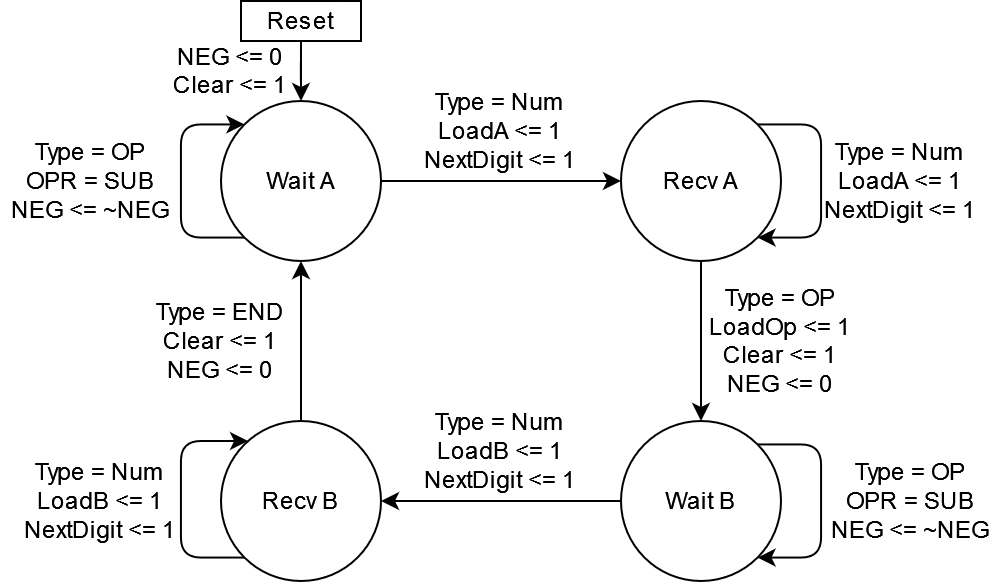
\includegraphics[width=.66\textwidth]{DecoderSM.drawio.png}
    \caption{ASCII Decoder Mealy State Machine Diagram}
    \label{fig:decodersm}
\end{figure} 


\subsection{Calculator}
% \begin{figure}[H]        
%     \centering
%     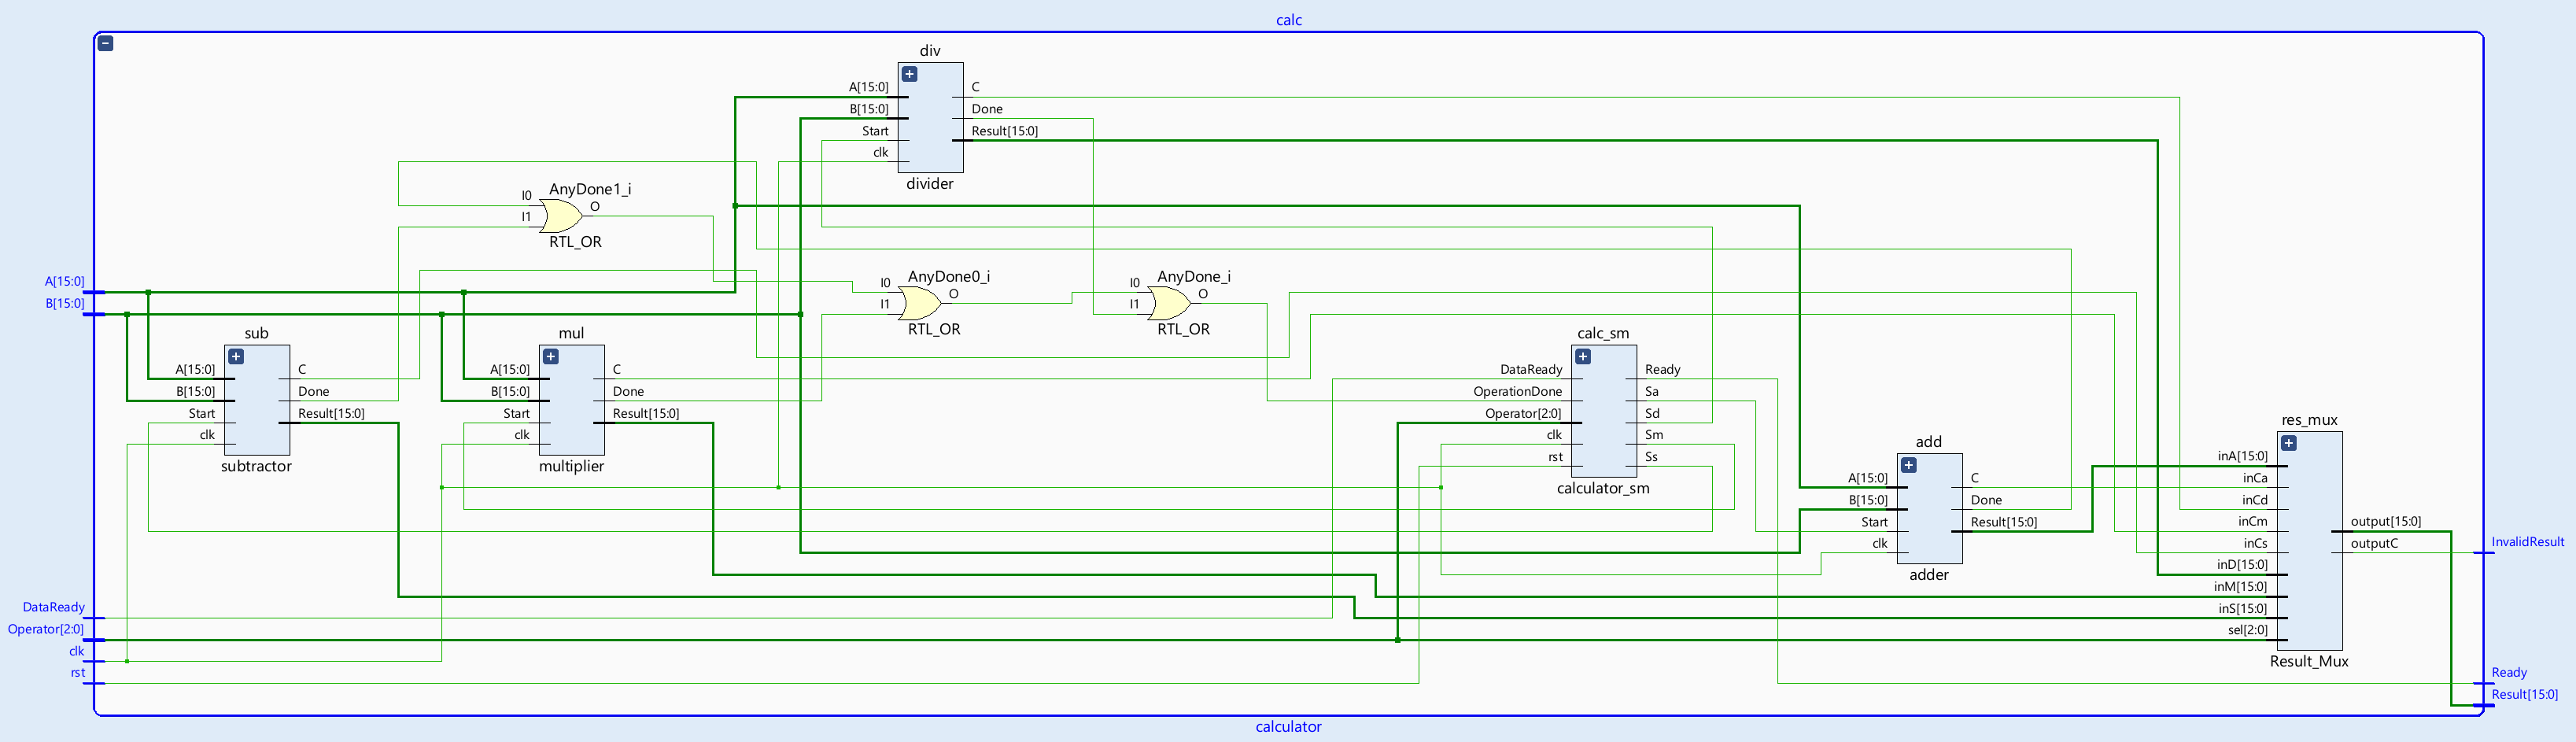
\includegraphics[width=\textwidth]{CalcImp.png}
%     \caption{Calculator Block Diagram}
%     \label{fig:calcimp}
% \end{figure} 

\begin{figure}[H]        
    \centering
    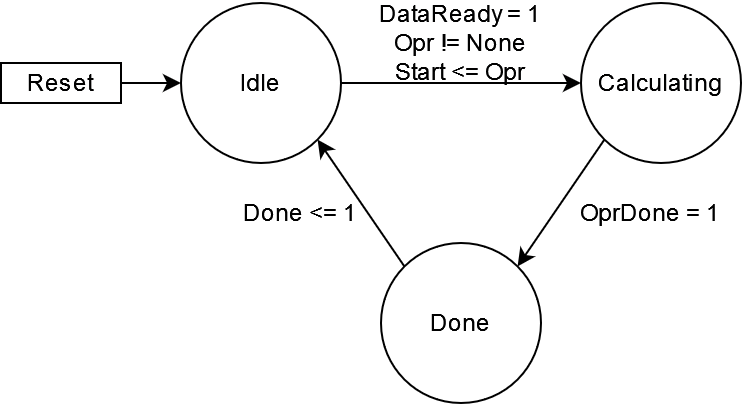
\includegraphics[width=.66\textwidth]{CalculatorSM.drawio.png}
    \caption{ASCII Calculator Mealy State Machine Diagram}
    \label{fig:calcsm}
\end{figure} 

\subsection{ASCII Encoder}
% \begin{figure}[H]        
%    \centering
%    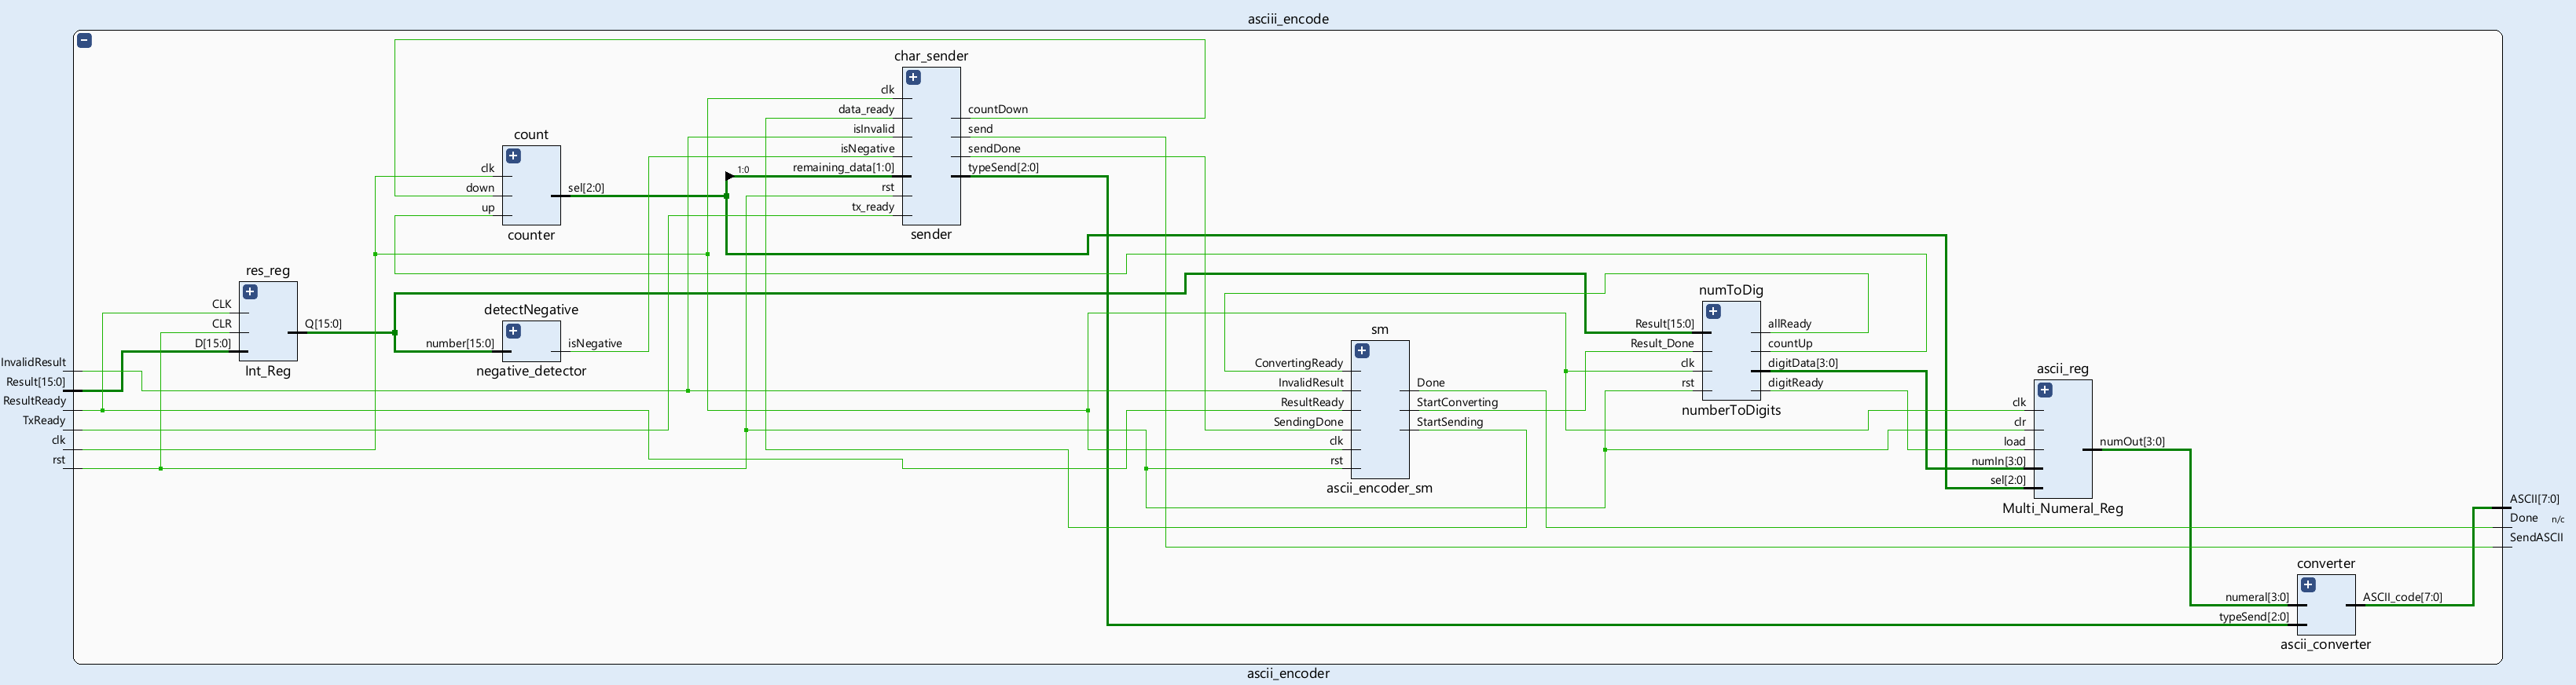
\includegraphics[width=\textwidth]{EncodeImp.png}
%    \caption{ASCII Encoder Block Diagram}
%    \label{fig:encoderimp}
% \end{figure} 

\begin{figure}[H]        
    \centering
    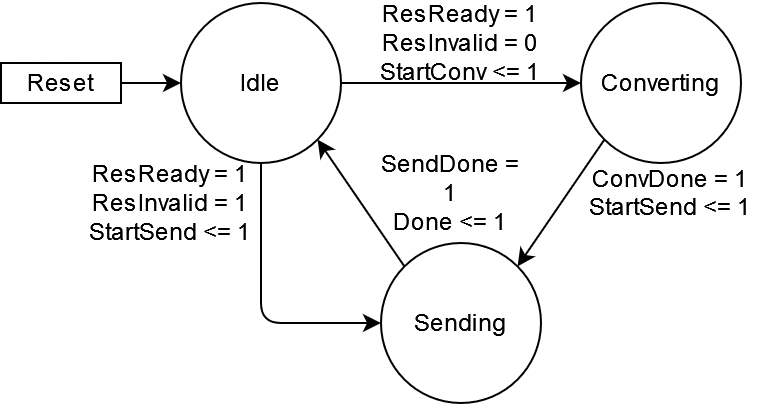
\includegraphics[width=.66\textwidth]{EncoderSM.drawio.png}
    \caption{ASCII Encoder Mealy State Machine Diagram}
    \label{fig:encodersm}
\end{figure} 

\subsubsection{Sender}
\begin{figure}[H]        
    \centering
    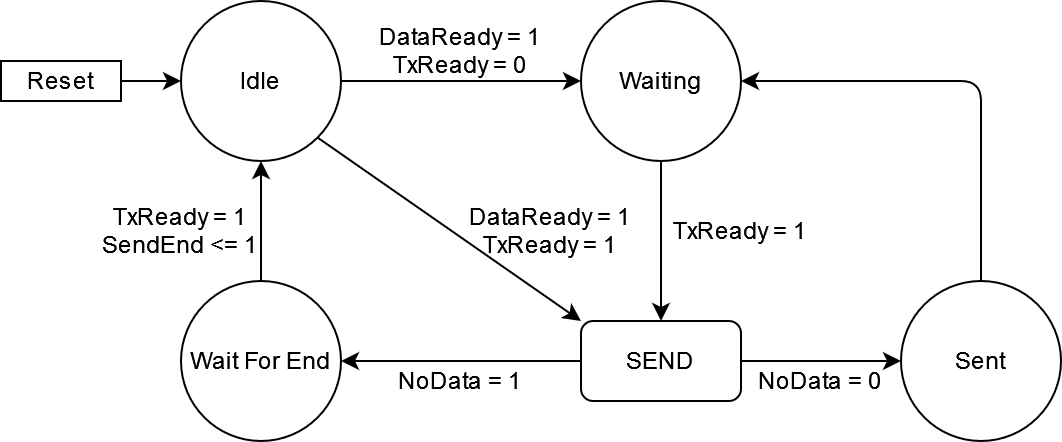
\includegraphics[width=.66\textwidth]{SenderSM.drawio.png}
    \caption{ASCII Sender Mealy State Machine Diagram}
    \label{fig:sendersm}
\end{figure} 


\subsection{Test Bench}
YOOOO


\section{Implementation}
\subsection{Timing}

\pagebreak
\printbibliography

\end{document}